\chapter{Rendezvous Value}
\section{Existence and Uniqueness}
The following theorem is due to Stadje \cite{stadje}. The special case of compact, connected, non-empty metric spaces had been formulated by Gross \cite{gross}, however, it appears that Stadje was unaware of the result from Gross.
\begin{theorem}[Gross-Stadje-Theorem]\label{thm:gross-stadje}
	Let $X$ be a compact, connected, non-empty Hausdorff space and $f: X\times X\to \R$ a continuous, symmetric function. Then there is a uniquely determined constant $a(X,f)\in\R$ such that the following holds:
	\begin{equation}\label{eq:def-average-distance}
	\forall n\in \N\quad\forall x_1,\dots,x_n\in X\quad \exists y\in X\colon \frac{1}{n}\sum_{i=1}^{n}f(x_i,y)=a(X,f).
	\end{equation}
\end{theorem}

Before we get started with the proof, let us examine a simple example. More advanced/interesting examples will be examined in a later chapter.
\begin{example}
	Let $(X,f):=([0,1],d)$ be the unit interval with the usual euclidean metric. Then $X$ is a compact connected hausdorff space and $d$ is a symmetric continuous function from $X\times X$ to $\R$.
	
	We consider the case of $n=2$ with $x_1=0$ and $x_2=1$:
	
	\begin{centering}
	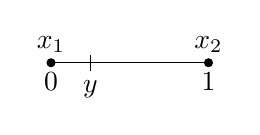
\begin{tikzpicture}[scale=2]
		\filldraw (0,0) circle(.25mm) node[below]{$0$} node[above]{$x_1$};
		\draw (0,0)--(1,0);
		\filldraw (1,0) circle(.25mm) node[below]{$1$} node[above]{$x_2$};
		\draw (0.25,0.05)--(0.25,-0.05) node[below]{$y$};
	\end{tikzpicture}
	
	\end{centering}
	
	It is elementary to see, that in this case $d(x_1,y)+d(x_2,y)\equiv 1$. Thus, if a rendezvous value for $([0,1],d)$ exists, then it has to be $\frac{1}{2}$.
\end{example}

\begin{proof}
	We will prove the existence of such a value by giving an explicit formula. However, it will be apparent, that this formula will not be particularly helpful for computing the rendezvous value of arbitrary spaces.
	
	Define
	\[
	a(X,f):=\sup_{\mu\in\M^1}\inf_{\nu\in\M^1} \int\limits_X\int\limits_X f(x,y)\mu(\dx)\nu(\dy).
	\]
	We now need to show that $a(X,f)$ actually satisfies \autoref{eq:def-average-distance}. As we saw in \autoref{thm:compactness},
	$\M^1(X)$ equipped with the weak*-topology is compact and the mapping $\mu\mapsto\int_Xf(x,y)\mu(\dx)$ is (lower semi-)continuous for each $y\in X$. 
	By minimax theorem (\autoref{thm:minimax}) we
	see 
	\[
	a(X,f)=\inf_{\nu\in\M^1}\sup_{\mu\in\M^1} \int\limits_X\int\limits_X f(x,y)\mu(\dx)\nu(\dy).
	\]
	
	For arbitrary points $x_1,\dots,x_n\in X$, we have
	\begin{align}\label{eq:sum-integral1}
		\sup_{y\in X}\frac{1}{n}\sum_{i=1}^{n}f(x_i,y)&\geq\sup_{y\in X}\inf_{\mu\in\M^1} \int\limits_X\int\limits_X f(x,y)\mu(\dx)=a(X,f),
		\\\label{eq:sum-integral2}
		\inf_{y\in X}\frac{1}{n}\sum_{i=1}^{n}f(x_i,y)&\leq\inf_{y\in X}\sup_{\mu\in\M^1} \int\limits_X\int\limits_X f(x,y)\mu(\dx)=a(X,f).
	\end{align}
	
	The mapping $y\overset{\phi}{\mapsto} \frac{1}{n}\sum_{i=1}^{n}f(x_i,y)$ is continuous since $f$ is continuous by assumption. 
	It is generally true, that the image of compact respectively connected spaces under continuous functions is again compact respectively connected. 
	This implies that the image $\mathrm{im}(\phi)$ is a compact interval in $\R$. Now it follows immediately form intermediate value theorem that there exists a $y\in X$ where equality holds in \autoref{eq:sum-integral1} and \ref{eq:sum-integral2}, i.e.
	\[
	\frac{1}{n}\sum_{i=1}^{n}f(x_i,y)=a(X,f).
	\]
	
	We shall now direct our attention towards the uniqueness of $a(X,f)$.
	Suppose there is another constant $a^\prime<a(X,f)$ satisfying \autoref{eq:def-average-distance} (The case of $a^\prime>a(X,f)$ is analogous). Choose $\alpha>0$ such that 
	\[
	a^\prime+3\alpha<\inf_\nu\sup_\mu\int_X\int_Xf(x,y)\nu(\dy)\mu(\dx)=\inf_y\sup_\mu\int_Xf(x,y)\mu(\dx)
	\]
	
	Since the probability measures with finite support are dense in $M^1(X)$ (see \autoref{thm:finite-support}) we can find $p_1,\dots,p_n\geq 0, \sum_{i=1}^{n}p_i=1$ and $x_1,\dots,x_n$, with the property
	\begin{equation}\label{eq:uniqueness-finite}
	a^\prime+2\alpha<\inf_y\sum_{i=1}^{n}p_if(x_i,y).
	\end{equation}
	
	Since
	\[
	\left|\sum_{i=1}^n p_if(x_i,y)-\sum_{i=1}^np_i^\prime f(x_i,y)\right|<\max_i |p_i-p_i^\prime|\sup_{x,y}|f(x,y)|,
	\]
	the right-hand side of \autoref{eq:uniqueness-finite} depends continuously on $(p_1,\dots,p_n)$.
	Consider for one moment the case of $p_i\in \mathbb{Q}$. Then there clearly exists $k,m_1,\dots,m_n\in N$ with $p_i=\frac{m_i}{k}$. Since $\mathbb{Q}$ is dense in $\R$ we find that even in the general case there exist $k, m_1,\dots,m_n\in \N$ satisfying
	\begin{equation}
		a^\prime +\alpha<\inf_y\frac{1}{k}\sum_{i=1}^{n}m_if(x_i,y),\quad \sum_{i=1}^nm_i=k.
	\end{equation}
	For the points
	\begin{align*}
	x_1^\prime=x_2^\prime=\cdots=x_{m_1}^\prime&:=x_1,
	\\
	x_{m_1+1}^\prime=\cdots=x_{m_2}^\prime&:=x_2,
	\\
	\vdots
	\\
	x_{k-m_n+1}^\prime=\cdots =x^\prime_k&:=x_n,
	\end{align*}
	there is no $y\in X$ such that \eqref{eq:def-average-distance} is valid with $x_i$ there replaced by $x_i^\prime$, $n$ by $k$ and $a$ by $a^\prime$. Hence $a(X,f)$ is uniquely determined.
\end{proof}


In the following paragraph we shall try to develop an intuition for the conditions under which above theorem holds.

It is quite obvious that $X$ actually has to be connected for this statement to hold, for otherwise consider the space $X=\{1,2\}\subset\R$ equipped with the subset Topology of $\R$ (this actually coincides with the discrete topology in this case). It is clear, that $X$ is compact and a Hausdorff space but not connected. Let $f$ be given by the euclidean metric.
Suppose $a(X,f)$ exists.
First, consider the situation, in which only one point is given. Then $y\in\{1,2\}$. So \[a(X,f)\in\left\{0,1\right\}=:A.\] Now consider the case where two points are given, in particular $\{x_1=1,x_2=2\}$. Again there are only two choices for $y$, however this gives $a(X,f)=\frac{1}{2}$ regardless of this choice. Since $\frac{1}{2}\not\in A$, we see that $a(X,f)$ can't exist.

Compactness is required in general to ensure that $a(X,f)$ is finite for all $f$ satisfying the assumptions.

%intuition for Hausdorff
%maybe with line with two zeros?

Note however, that no claim was made whether \autoref{thm:gross-stadje} can be generalized to a broader category of spaces or not. We will actually discuss spheres in Banach spaces in \autoref{chap:further}, which are only compact if the dimension is finite.


\begin{corollary}\label{cor:continuous}
	Let $X$ be a compact, connected, non-empty Hausdorff space and let $C_s(X,\R)$ be the set of symmetric continuous functions from $X$ to $\R$ equipped with the uniform topology. The function
	\begin{align*}
		C_s(X,\R)&\to \R
		\\
		f&\mapsto a(X,f)
	\end{align*}
	is continuous.
\end{corollary}

\begin{proof}
	Recall form the proof of \autoref{thm:gross-stadje} we have the formula\[
	a(X,f)=\inf_{\nu\in\M^1}\sup_{\mu\in\M^1}\int_X\int_X f(x,y)\nu(\dy)\mu(\dx)
	\]
%	
%	The statement follows now since we can exchange the limit with taking the infimum and supremum since the mappings 
%	\begin{align*}
%		\mu&\mapsto \int_X f(x,y)\mu(\dx)\quad \forall y\in X\\
%		\nu&\mapsto \sup_{\mu\in\M^1}\int_X\int_Xf(x,y)\mu(\dx)\nu(\dy)\quad \forall \mu\in \M^1(X)
%	\end{align*}
%	are continuous. We can further exchange taking the limit and integration since we equipped $C_s(X,\R)$ with the uniform topology.
%%TODO elaborate
Now consider $f,g\in C_s(X,\R)$ with $\sup_{x,y}|f(x,y)-g(x,y)|<\varepsilon$ for some $\varepsilon>0$, then for all $\mu,\nu\in \M^1$:
\begin{align*}
	\int_X\int_Xg(x,y)\mu(\dx)\nu(\dy)-\varepsilon&\leq\int_X\int_Xf(x,y)\mu(\dx)\nu(\dy)\\
	&\leq\int_X\int_X(x,y)\mu(\dx)\nu(\dy)+\varepsilon.
\end{align*}
Applying $\inf$ and $\sup$ consecutively results in
\[
a(X,g)-\varepsilon\leq a(X,f)\leq a(X,g)+\varepsilon,
\]
hence the described mapping is continuous with respect to the uniform topology on $C_s(X,\R)$.
\end{proof}